\chapter{怎样克服自激振荡}\label{ch5}
\section{自激振荡是怎么回事?}
\section{内部反射引起的自激振荡}
\section{外部反馈引起的自激振荡}
\section{二次电子引起的自激振荡}
\section{怎样判断自激振荡?}







\begin{figure}[phtb]
	\centering
	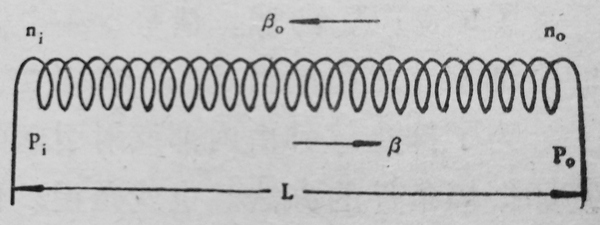
\includegraphics[width=0.65\linewidth]{figure/ch5-1}
	\caption{内部反射引起自激振荡的振幅条件$ G>\frac{L}{n_i n_o} $}
	\label{ch5-1}
\end{figure}

\begin{figure}[phtb]
\centering
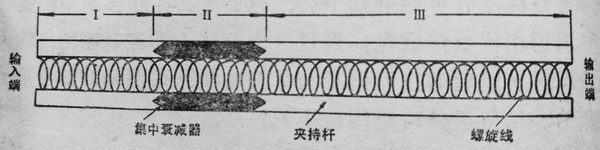
\includegraphics[width=0.65\linewidth]{figure/ch5-2}
\caption{行波管中的集中衰减器}
\label{ch5-2}
\end{figure}

\begin{figure}[phtb]
	\centering
	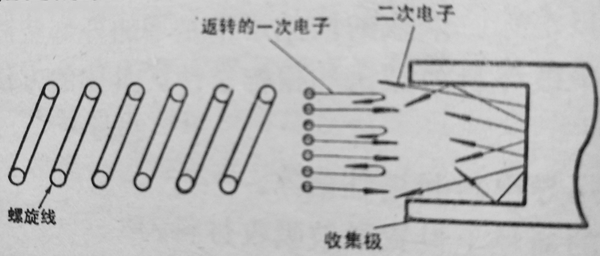
\includegraphics[width=0.65\linewidth]{figure/ch5-3}
	\caption{二次电子和反转的一次电子进入螺旋线}
	\label{ch5-3}
\end{figure}

\begin{figure}[phtb]
	\centering
	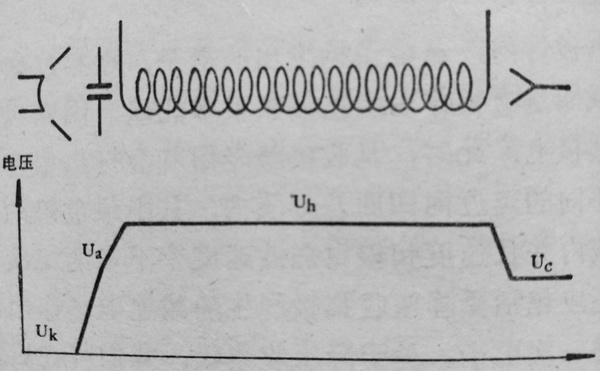
\includegraphics[width=0.65\linewidth]{figure/ch5-4}
	\caption{收集极降压行波管的电位分布}
	\label{ch5-4}
\end{figure}

\begin{figure}[phtb]
	\centering
	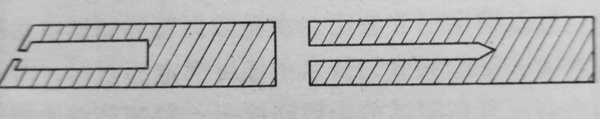
\includegraphics[width=0.65\linewidth]{figure/ch5-5}
	\caption{改进收集极结构}
	\label{ch5-5}
\end{figure}

\begin{figure}[phtb]
	\centering
	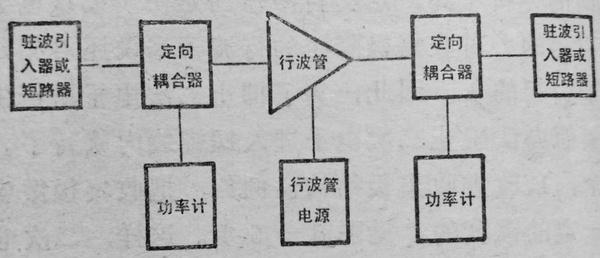
\includegraphics[width=0.65\linewidth]{figure/ch5-6}
	\caption{行波管自激振荡测试方框图}
	\label{ch5-6}
\end{figure}